\documentclass[11pt,a4paper]{report}
\usepackage[textwidth=37em,vmargin=30mm]{geometry}
\usepackage{calc,xunicode,amsmath,amssymb,paralist,enumitem,tabu,booktabs,datetime2,xeCJK,xeCJKfntef,listings}
\usepackage{tocloft,fancyhdr,tcolorbox,xcolor,graphicx,eso-pic,xltxtra,xelatexemoji}

\newcommand{\envyear}[0]{2025}
\newcommand{\envdatestr}[0]{2025-03-10}
\newcommand{\envfinaldir}[0]{webdb/2025/20250310/final}

\usepackage[hidelinks]{hyperref}
\hypersetup{
    colorlinks=false,
    pdfpagemode=FullScreen,
    pdftitle={Web Digest - \envdatestr}
}

\setlength{\cftbeforechapskip}{10pt}
\renewcommand{\cftchapfont}{\rmfamily\bfseries\large\raggedright}
\setlength{\cftbeforesecskip}{2pt}
\renewcommand{\cftsecfont}{\sffamily\small\raggedright}

\setdefaultleftmargin{2em}{2em}{1em}{1em}{1em}{1em}

\usepackage{xeCJK,xeCJKfntef}
\xeCJKsetup{PunctStyle=plain,RubberPunctSkip=false,CJKglue=\strut\hskip 0pt plus 0.1em minus 0.05em,CJKecglue=\strut\hskip 0.22em plus 0.2em}
\XeTeXlinebreaklocale "zh"
\XeTeXlinebreakskip = 0pt


\setmainfont{Brygada 1918}
\setromanfont{Brygada 1918}
\setsansfont{IBM Plex Sans}
\setmonofont{JetBrains Mono NL}
\setCJKmainfont{Noto Serif CJK SC}
\setCJKromanfont{Noto Serif CJK SC}
\setCJKsansfont{Noto Sans CJK SC}
\setCJKmonofont{Noto Sans CJK SC}

\setlength{\parindent}{0pt}
\setlength{\parskip}{8pt}
\linespread{1.15}

\lstset{
	basicstyle=\ttfamily\footnotesize,
	numbersep=5pt,
	backgroundcolor=\color{black!5},
	showspaces=false,
	showstringspaces=false,
	showtabs=false,
	tabsize=2,
	captionpos=b,
	breaklines=true,
	breakatwhitespace=true,
	breakautoindent=true,
	linewidth=\textwidth
}






\newcommand{\coverpic}[2]{
    % argv: itemurl, authorname
    Cover photo by #2~~(\href{#1}{#1})
}
\newcommand{\makeheader}[0]{
    \begin{titlepage}
        % \newgeometry{hmargin=15mm,tmargin=21mm,bmargin=12mm}
        \begin{center}
            
            \rmfamily\scshape
            \fontspec{BaskervilleF}
            \fontspec{Old Standard}
            \fontsize{59pt}{70pt}\selectfont
            WEB\hfill DIGEST
            
            \vfill
            % \vskip 30pt
            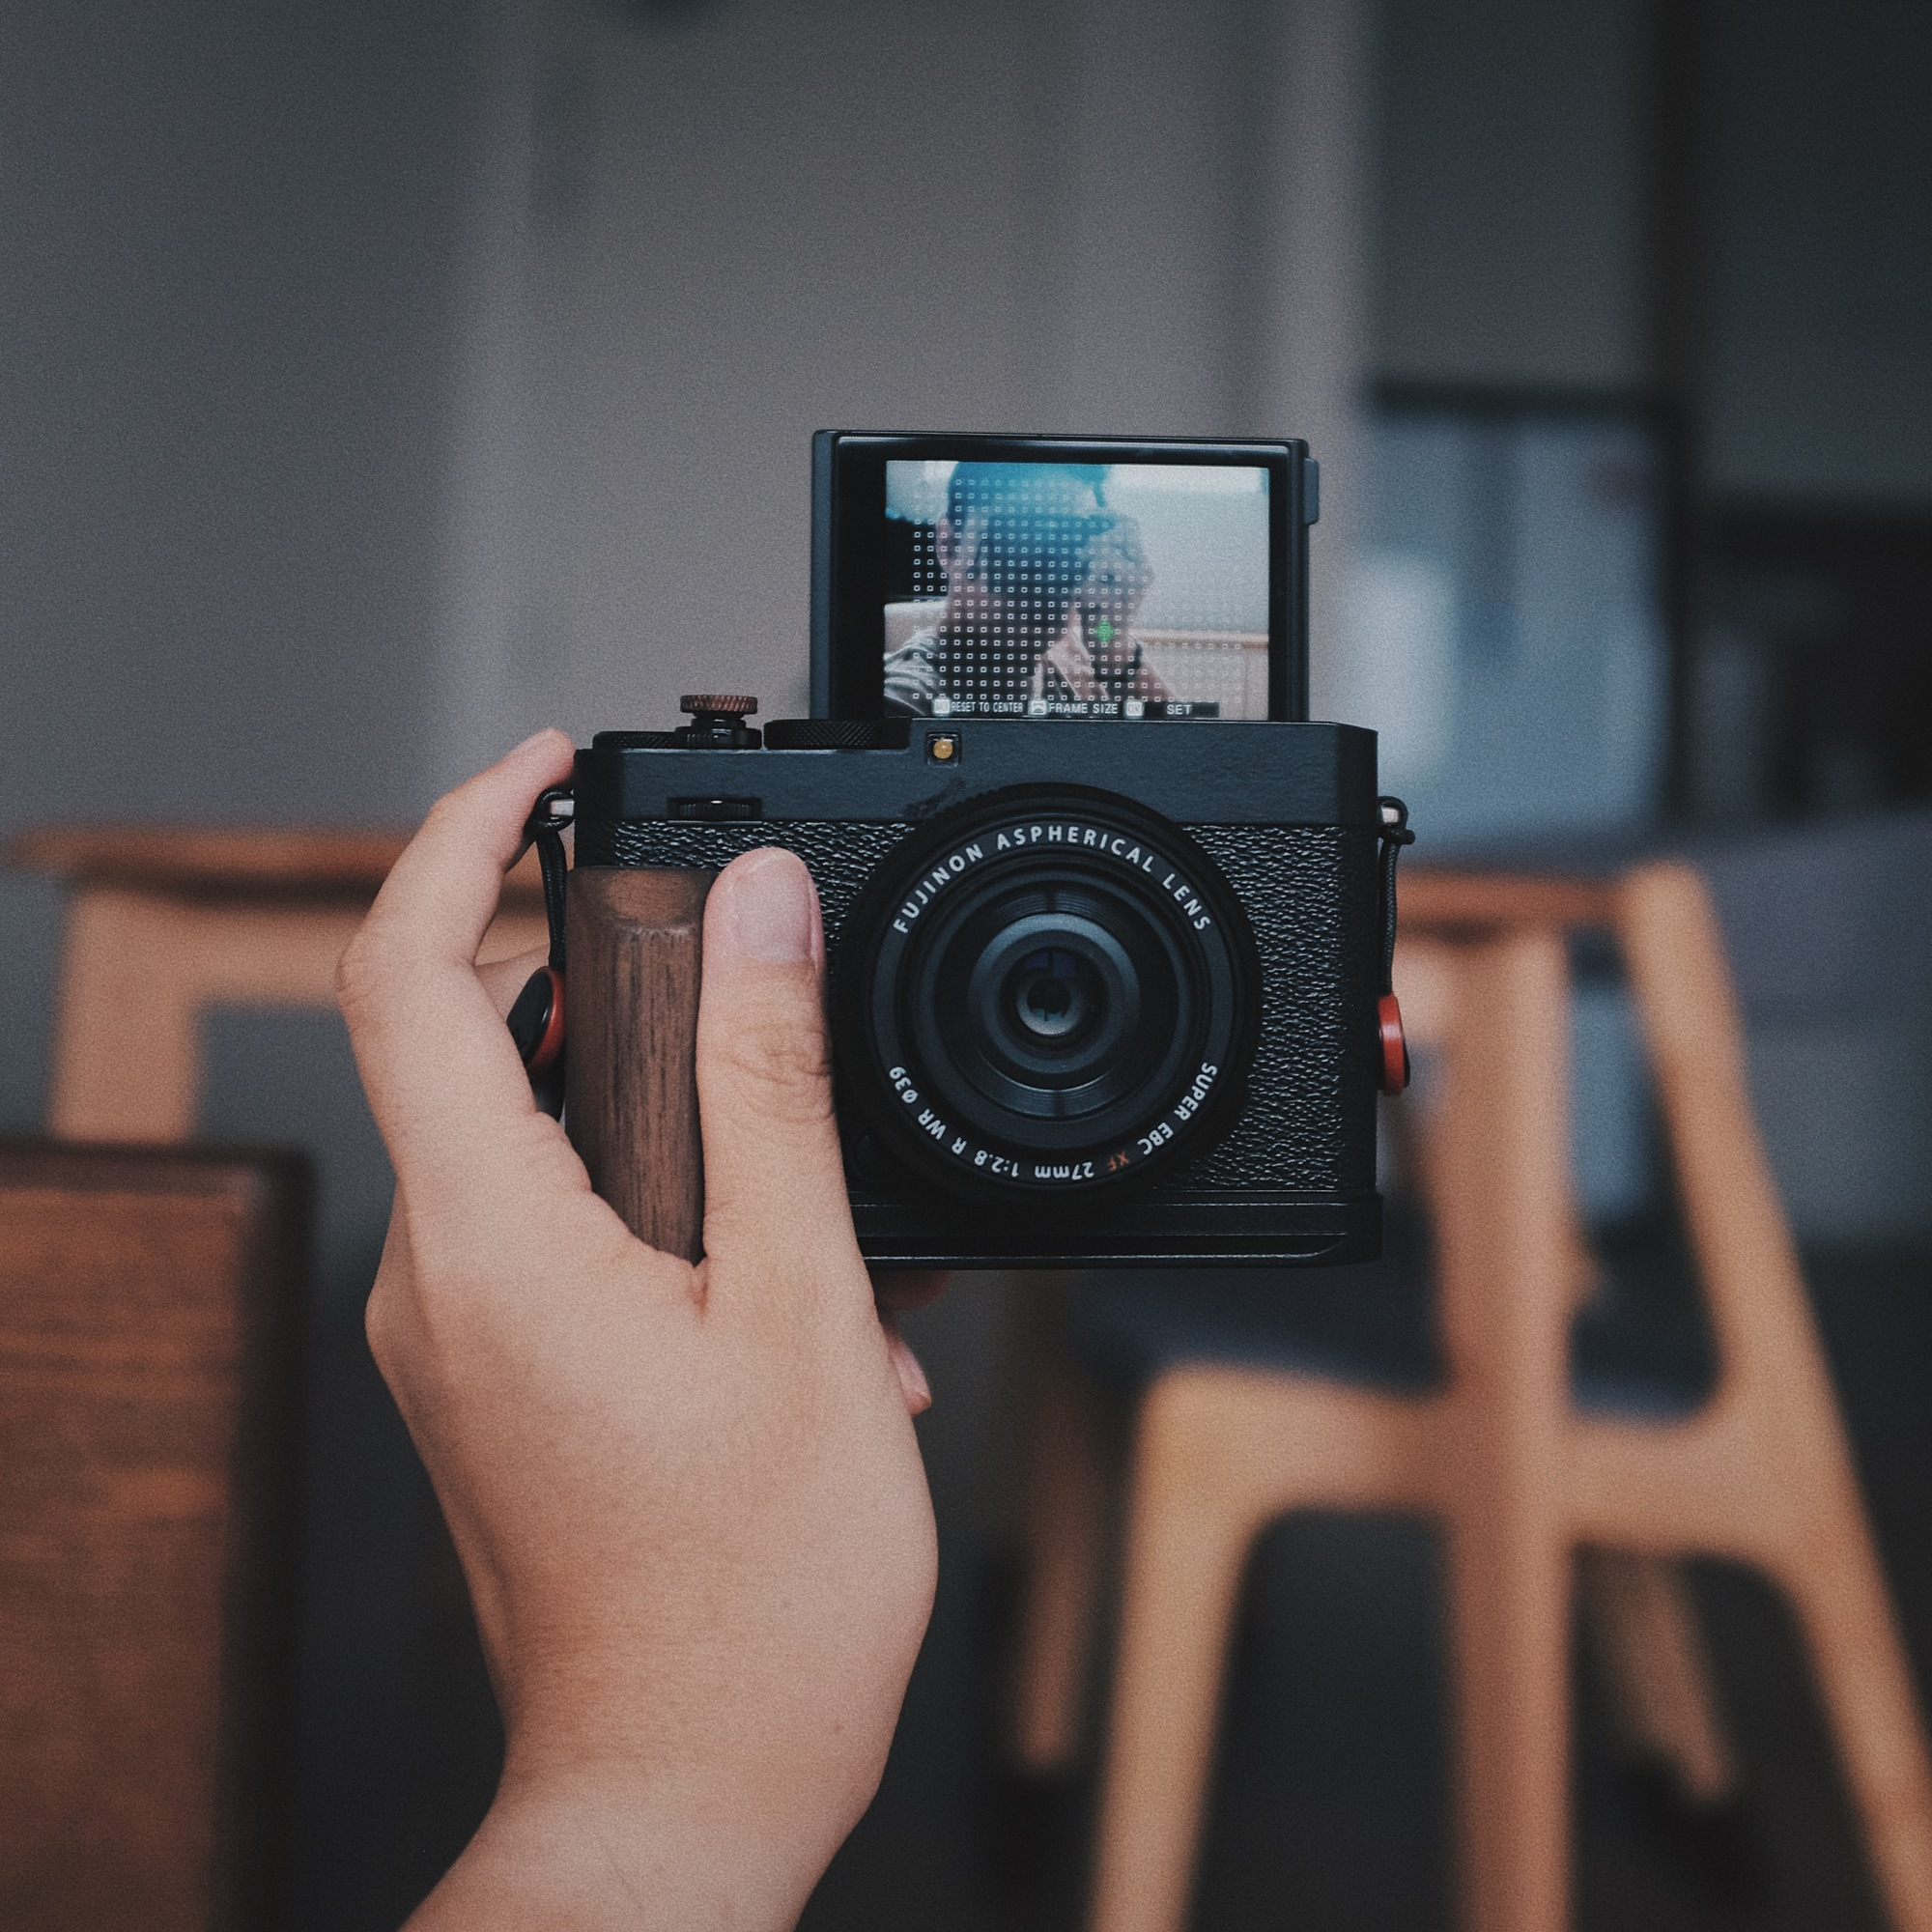
\includegraphics[width=\linewidth]{\envfinaldir/coverpic-prod.jpg}\par
            % \vskip 30pt
            \vfill

            \normalsize\rmfamily\scshape
            \copyright{} The Web Digest Project \hfill\large \envdatestr
        \end{center}
    \end{titlepage}
    % \restoregeometry
}
\newcommand{\simplehref}[1]{%
    \textcolor{blue!80!green}{\href{#1}{#1}}%
}
\renewcommand{\contentsname}{\center\Huge\sffamily\bfseries Contents\par\vskip 20pt}
\newcounter{ipartcounter}
\setcounter{ipartcounter}{0}
\newcommand{\ipart}[1]{
    % \vskip 20pt
    \clearpage
    \stepcounter{ipartcounter}
    \phantomsection
    \addcontentsline{toc}{chapter}{#1}
    % \begin{center}
    %     \Huge
    %     \sffamily\bfseries
    %     #1
    % \end{center}
    % \vskip 20pt plus 7pt
}
\newcounter{ichaptercounter}
\setcounter{ichaptercounter}{0}
\newcommand{\ichapter}[1]{
    % \vskip 20pt
    \clearpage
    \stepcounter{ichaptercounter}
    \phantomsection
    \addcontentsline{toc}{section}{\numberline{\arabic{ichaptercounter}}#1}
    \begin{center}
        \Huge
        \sffamily\bfseries
        #1
    \end{center}
    \vskip 20pt plus 7pt
}
\newcommand{\entrytitlefont}[1]{\subsection*{\raggedright\Large\sffamily\bfseries#1}}
\newcommand{\entryitemGeneric}[2]{
    % argv: title, url
    \parbox{\linewidth}{
        \entrytitlefont{#1}\par\vskip 5pt
        \footnotesize\ttfamily\mdseries
        \simplehref{#2}
    }\vskip 11pt plus 11pt minus 1pt
}
\newcommand{\entryitemGithub}[3]{
    % argv: title, url, desc
    \parbox{\linewidth}{
        \entrytitlefont{#1}\par\vskip 5pt
        \footnotesize\ttfamily\mdseries
        \simplehref{#2}\par\vskip 5pt
        \small\rmfamily\mdseries#3
    }\vskip 11pt plus 11pt minus 1pt
}
\newcommand{\entryitemAp}[3]{
    % argv: title, url, desc
    \parbox{\linewidth}{
        \entrytitlefont{#1}\par\vskip 5pt
        \footnotesize\ttfamily\mdseries
        \simplehref{#2}\par\vskip 5pt
        \small\rmfamily\mdseries#3
    }\vskip 11pt plus 11pt minus 1pt
}
\newcommand{\entryitemHackernews}[3]{
    % argv: title, hnurl, rawurl
    % \parbox{\linewidth}{
    %     \entrytitlefont{#1}\par\vskip 5pt
    %     \footnotesize\ttfamily\mdseries
    %     \simplehref{#3}\par
    %     \textcolor{black!50}{\href{#2}{#2}}
    % }\vskip 11pt plus 11pt minus 1pt
    \begin{minipage}{\linewidth}
            \entrytitlefont{#1}\par\vskip 5pt
            \footnotesize\ttfamily\mdseries
            \simplehref{#3}\par
            \textcolor{black!50}{\href{#2}{#2}}
    \end{minipage}\par\vskip 11pt plus 11pt minus 1pt
}







\begin{document}

\makeheader

\tableofcontents\clearpage




\ipart{Developers}
\ichapter{Hacker News}
\entryitemTwoLinks{Tesla Sales Fall Off a Cliff Globally, Including Germany, Australia, and China}{https://news.ycombinator.com/item?id=43313127}{https://www.carscoops.com/2025/03/tesla-sales-falling-off-a-cliff-globally-including-germany-australia-and-china/}

\entryitemTwoLinks{Europe bets once again on RISC-V for supercomputing}{https://news.ycombinator.com/item?id=43311091}{https://www.theregister.com/2025/03/07/dare\_europe\_risc\_v\_project/}

\entryitemTwoLinks{It is as if you were on your phone}{https://news.ycombinator.com/item?id=43308994}{https://pippinbarr.com/it-is-as-if-you-were-on-your-phone/info/}

\entryitemTwoLinks{US Ends Support For Ukrainian F-16s}{https://news.ycombinator.com/item?id=43307996}{https://ukrainetoday.org/us-ends-support-for-ukrainian-f-16s-but-french-mirages-will-be-salvation-forbes/}

\entryitemTwoLinks{Gleam v1.9}{https://news.ycombinator.com/item?id=43307987}{https://gleam.run/news/hello-echo-hello-git/}

\entryitemTwoLinks{I've been using Claude Code for a couple of days}{https://news.ycombinator.com/item?id=43307809}{https://twitter.com/Steve\_Yegge/status/1898674257808515242}

\entryitemTwoLinks{Layoffs Don't Work}{https://news.ycombinator.com/item?id=43307755}{https://thehustle.co/originals/why-layoffs-dont-work}

\entryitemTwoLinks{Goravel: A Go framework inspired by Laravel}{https://news.ycombinator.com/item?id=43306797}{https://www.goravel.dev}

\entryitemTwoLinks{Stem cell therapy trial reverses "irreversible" damage to cornea}{https://news.ycombinator.com/item?id=43306734}{https://newatlas.com/biology/stem-cell-therapy-reverses-irreversible-damage-cornea/}

\entryitemTwoLinks{Magnesium Self-Experiments}{https://news.ycombinator.com/item?id=43306599}{https://gwern.net/nootropic/magnesium}

\entryitemTwoLinks{A Post Mortem on the Gino Case}{https://news.ycombinator.com/item?id=43306435}{https://statmodeling.stat.columbia.edu/2025/03/08/a-post-mortem-on-the-gino-case-committing-fraud-is-right-now-a-viable-career-strategy-that-can-propel-you-at-the-top-of-the-academic-world/}

\entryitemTwoLinks{Online Embedded Rust Simulator}{https://news.ycombinator.com/item?id=43305973}{https://wokwi.com/rust}

\entryitemTwoLinks{Posthog/.cursorrules}{https://news.ycombinator.com/item?id=43305919}{https://github.com/PostHog/posthog/blob/master/.cursorrules}

\entryitemTwoLinks{My 16-month theanine self-experiment}{https://news.ycombinator.com/item?id=43305803}{https://dynomight.net/theanine/}

\entryitemTwoLinks{Building an open-source Wi-Fi Mac layer for the ESP32}{https://news.ycombinator.com/item?id=43304962}{https://esp32-open-mac.be}

\entryitemTwoLinks{Show HN: I built an app to get daily wisdom from Mr. Worldwide}{https://news.ycombinator.com/item?id=43304785}{https://daale.club/}

\entryitemTwoLinks{Stuff a Pi-hole in your router because your browser is about to betray you}{https://news.ycombinator.com/item?id=43303922}{https://www.theregister.com/2025/03/08/pi\_hole\_6\_flyby/}

\entryitemTwoLinks{Presenterm: Markdown Slideshows in the Terminal}{https://news.ycombinator.com/item?id=43303752}{https://github.com/mfontanini/presenterm}

\entryitemTwoLinks{Deploy from local to production (self-hosted)}{https://news.ycombinator.com/item?id=43302495}{https://github.com/bypirob/airo}

\entryitemTwoLinks{MCP vs. API Explained}{https://news.ycombinator.com/item?id=43302297}{https://norahsakal.com/blog/mcp-vs-api-model-context-protocol-explained/}\ichapter{Phoronix}
\entryitemGeneric{\hskip 0pt{}AMD Preparing "High Precision" Mode For Upcoming Instinct MI350X (GFX950)}{https://www.phoronix.com/news/AMD-HSA-High-Precision-MI350X}

\entryitemGeneric{\hskip 0pt{}Intel Preps Linux For "Platform Temperature Control" With Lunar Lake \& Panther Lake SoCs}{https://www.phoronix.com/news/Intel-PTC-Linux-Lunar-Panther}

\entryitemGeneric{\hskip 0pt{}More Apple Silicon Updates For Linux 6.15 Help M1/M2 Plus iPad / iPod / iPhone}{https://www.phoronix.com/news/Apple-Silicon-DT-3-Linux-6.15}

\entryitemGeneric{\hskip 0pt{}ALGOL 68 Compiler Front-End Not Being Merged Into GCC At This Point}{https://www.phoronix.com/news/ALGOL-68-No-GCC-2025}

\entryitemGeneric{\hskip 0pt{}Intel NPU Firmware Files Upstreamed To linux-firmware.git}{https://www.phoronix.com/news/Intel-NPU-Firmware-Upstream}

\entryitemGeneric{\hskip 0pt{}Wine Releases Framework Mono 6.14 In Taking Over The Mono Project}{https://www.phoronix.com/news/Wine-Framework-Mono-6.14}

\entryitemGeneric{\hskip 0pt{}Rust Coreutils 0.0.30 Enhances GNU Compatibility, Uutils To Port More Common Unix Tools}{https://www.phoronix.com/news/uutils-Coreutils-0.0.30}

\entryitemGeneric{\hskip 0pt{}GTK On Android \& macOS Seeing Improvements}{https://www.phoronix.com/news/GNOME-GTK-Android-macOS}

\entryitemGeneric{\hskip 0pt{}Mesa's Venus Driver Adds Vulkan Ray-Tracing Support For VMs}{https://www.phoronix.com/news/Mesa-25.1-Venus-Vulkan-RT}\ichapter{Dribbble}
\entryitemGeneric{\hskip 0pt{}Free Fly Apparel}{https://dribbble.com/shots/25727838-Free-Fly-Apparel}

\entryitemGeneric{\hskip 0pt{}Columbus Rapids® C-Wave}{https://dribbble.com/shots/25727535-Columbus-Rapids-C-Wave}

\entryitemGeneric{\hskip 0pt{}Bloodhound Detective}{https://dribbble.com/shots/25726401-Bloodhound-Detective}

\entryitemGeneric{\hskip 0pt{}QLOUD - Logo Redesign}{https://dribbble.com/shots/25726630-QLOUD-Logo-Redesign}

\entryitemGeneric{\hskip 0pt{}Faithful web design}{https://dribbble.com/shots/25723024-Faithful-web-design}

\entryitemGeneric{\hskip 0pt{}Logo Design for Streaming Platform (Unused for Sale)}{https://dribbble.com/shots/25726051-Logo-Design-for-Streaming-Platform-Unused-for-Sale}

\entryitemGeneric{\hskip 0pt{}Dj Dule logo}{https://dribbble.com/shots/25725864-Dj-Dule-logo}

\entryitemGeneric{\hskip 0pt{}Puzzle Fintech Website Design}{https://dribbble.com/shots/25651990-Puzzle-Fintech-Website-Design}

\entryitemGeneric{\hskip 0pt{}Dashboard for an Education Product ✦ Golf Pro}{https://dribbble.com/shots/25720487-Dashboard-for-an-Education-Product-Golf-Pro}

\entryitemGeneric{\hskip 0pt{}Proboscis Monkey}{https://dribbble.com/shots/25720978-Proboscis-Monkey}

\entryitemGeneric{\hskip 0pt{}Logofolio Update - March 2025}{https://dribbble.com/shots/25719985-Logofolio-Update-March-2025}

\entryitemGeneric{\hskip 0pt{}Bento grid barbershop platform UI}{https://dribbble.com/shots/25715947-Bento-grid-barbershop-platform-UI}

\entryitemGeneric{\hskip 0pt{}Cimet Slogan}{https://dribbble.com/shots/25710581-Cimet-Slogan}

\entryitemGeneric{\hskip 0pt{}Real Estate Platform UI}{https://dribbble.com/shots/25711538-Real-Estate-Platform-UI}

\entryitemGeneric{\hskip 0pt{}Logistics Company Web Design Landing Page}{https://dribbble.com/shots/25708252-Logistics-Company-Web-Design-Landing-Page}

\entryitemGeneric{\hskip 0pt{}Easy A Deck}{https://dribbble.com/shots/25715917-Easy-A-Deck}

\entryitemGeneric{\hskip 0pt{}Letter C + Hummingbird}{https://dribbble.com/shots/25713900-Letter-C-Hummingbird}

\entryitemGeneric{\hskip 0pt{}Inner Truth}{https://dribbble.com/shots/25659901-Inner-Truth}

\entryitemGeneric{\hskip 0pt{}Landing Page: AI Testing}{https://dribbble.com/shots/25714074-Landing-Page-AI-Testing}

\entryitemGeneric{\hskip 0pt{}Star + Check Mark Icon Concept}{https://dribbble.com/shots/25709690-Star-Check-Mark-Icon-Concept}

\entryitemGeneric{\hskip 0pt{}FREELANCE (Finally)}{https://dribbble.com/shots/25710537-FREELANCE-Finally}

\entryitemGeneric{\hskip 0pt{}Recent Logo Designs - Jeroen van Eerden}{https://dribbble.com/shots/25709914-Recent-Logo-Designs-Jeroen-van-Eerden}

\entryitemGeneric{\hskip 0pt{}Wolf}{https://dribbble.com/shots/25707625-Wolf}

\entryitemGeneric{\hskip 0pt{}Boletus logo}{https://dribbble.com/shots/25709349-Boletus-logo}


\ipart{Developers~~~~(zh-Hans)}
\ichapter{Solidot}
\entryitemGeneric{\hskip 0pt{}印度女性每天在无偿家务上的时间两倍多于男性}{https://www.solidot.org/story?sid=80738}

\entryitemGeneric{\hskip 0pt{}巴西法官命令苹果在 90 天内开放其 iOS 平台}{https://www.solidot.org/story?sid=80737}

\entryitemGeneric{\hskip 0pt{}微软开发与 OpenAI 竞争的大模型 MAI}{https://www.solidot.org/story?sid=80736}

\entryitemGeneric{\hskip 0pt{}柯伊伯带可能有很多三体系统}{https://www.solidot.org/story?sid=80735}

\entryitemGeneric{\hskip 0pt{}Intuitive Machines 的雅典娜月球探测器因侧翻而提前终止任务}{https://www.solidot.org/story?sid=80734}

\entryitemGeneric{\hskip 0pt{}天文学家认为一颗垂死恒星发出的神秘信号源自被撕裂的行星}{https://www.solidot.org/story?sid=80733}

\entryitemGeneric{\hskip 0pt{}周末前做手术有更高的死亡和并发症风险}{https://www.solidot.org/story?sid=80732}

\entryitemGeneric{\hskip 0pt{}研究人员从拉布拉多身上发现人犬共享肥胖相关基因}{https://www.solidot.org/story?sid=80731}\ichapter{V2EX}
\entryitemGeneric{\hskip 0pt{}[程序员] 面向海外华人独立站推广}{https://www.v2ex.com/t/1117118}

\entryitemGeneric{\hskip 0pt{}[分享创造] 用 cursor 写了个 ripgrep 的 GUI 界面}{https://www.v2ex.com/t/1117117}

\entryitemGeneric{\hskip 0pt{}[Apple] iOS 18.4 beta2 支付宝碰一碰无法使用}{https://www.v2ex.com/t/1117116}

\entryitemGeneric{\hskip 0pt{}[macOS] 请教一下大佬们, 黑苹果(Hackintosh)用什么显卡最合适?}{https://www.v2ex.com/t/1117115}

\entryitemGeneric{\hskip 0pt{}[问与答] [咨询]预算 10 万以内,打算给老爸弄一个 SUV 油车}{https://www.v2ex.com/t/1117114}

\entryitemGeneric{\hskip 0pt{}[程序员] 疯了😂RTX3090 涡轮公版的风扇转速怎么控制}{https://www.v2ex.com/t/1117113}

\entryitemGeneric{\hskip 0pt{}[问与答] 关于 yandex 以图搜图功能维护中}{https://www.v2ex.com/t/1117112}

\entryitemGeneric{\hskip 0pt{}[日本] 最近几天在日本,过几天回国,有需要代购的吗?}{https://www.v2ex.com/t/1117111}

\entryitemGeneric{\hskip 0pt{}[Apple] 记录并分享一下 macOS 优化提速脚本}{https://www.v2ex.com/t/1117110}

\entryitemGeneric{\hskip 0pt{}[问与答] 新入职的一个公司需要自己带笔记本电脑,求二手办公本推荐}{https://www.v2ex.com/t/1117109}

\entryitemGeneric{\hskip 0pt{}[程序员] 自己的第一个开源项目 db2llm}{https://www.v2ex.com/t/1117108}

\entryitemGeneric{\hskip 0pt{}[分享创造] [旅行 APP 产品诞生日记] 12day/100days}{https://www.v2ex.com/t/1117107}

\entryitemGeneric{\hskip 0pt{}[C++] 使用 C++20 协程与 ASIO 库写了个 Socks5 Server 的跨平台 Demo 程序,几乎全功能,单文件源码少于一千行}{https://www.v2ex.com/t/1117106}

\entryitemGeneric{\hskip 0pt{}[问与答] 33 岁失业设计师香氛创业 2 周年自我访谈分享}{https://www.v2ex.com/t/1117105}

\entryitemGeneric{\hskip 0pt{}[问与答] 自托管私有网络的 vaultwarden server, bitwarden 无法离线保存东西}{https://www.v2ex.com/t/1117104}

\entryitemGeneric{\hskip 0pt{}[分享创造] 发现一个可以直接生成 videoObject 的工具}{https://www.v2ex.com/t/1117102}

\entryitemGeneric{\hskip 0pt{}[分享发现] 智能适配}{https://www.v2ex.com/t/1117100}

\entryitemGeneric{\hskip 0pt{}[问与答] 英文 pdf 翻译。}{https://www.v2ex.com/t/1117097}

\entryitemGeneric{\hskip 0pt{}[Apple] 求购 MACBook 想求购一台 16+512 的 19-20 年的}{https://www.v2ex.com/t/1117095}

\entryitemGeneric{\hskip 0pt{}[问与答] Orz ,求推荐 广佛地区的数字游民社区。打算临时住一周。}{https://www.v2ex.com/t/1117094}

\entryitemGeneric{\hskip 0pt{}[OpenAI] deepseek 这个``服务器繁忙''是只对免费用户的吧?}{https://www.v2ex.com/t/1117093}

\entryitemGeneric{\hskip 0pt{}[问与答] 纯好奇:这年头 CSDN 到底哪儿好用?}{https://www.v2ex.com/t/1117092}

\entryitemGeneric{\hskip 0pt{}[macOS] macOS 连续输错 33 次开机密码还没被锁定!?}{https://www.v2ex.com/t/1117091}

\entryitemGeneric{\hskip 0pt{}[程序员] PHP 项目有类似前端 monorepo 的概念吗?}{https://www.v2ex.com/t/1117090}

\entryitemGeneric{\hskip 0pt{}[问与答] Cloudflare Tunnel 连不上了}{https://www.v2ex.com/t/1117089}

\entryitemGeneric{\hskip 0pt{}[微信] 有没有汇总微信每个版本的更新日志的地方?}{https://www.v2ex.com/t/1117088}

\entryitemGeneric{\hskip 0pt{}[Android] B 站 neo10 pro 的屏幕评测是不是广?护眼层面对比 k80 如何?}{https://www.v2ex.com/t/1117087}

\entryitemGeneric{\hskip 0pt{}[生活] 奇葩丈母娘干涉育儿教育}{https://www.v2ex.com/t/1117086}

\entryitemGeneric{\hskip 0pt{}[程序员] Cursor 到底比 VSCode+Copilot 强在哪?求指导}{https://www.v2ex.com/t/1117083}

\entryitemGeneric{\hskip 0pt{}[Windows] 为什么就任务管理器是糊的}{https://www.v2ex.com/t/1117082}

\entryitemGeneric{\hskip 0pt{}[问与答] 执行力差怎么办?}{https://www.v2ex.com/t/1117081}

\entryitemGeneric{\hskip 0pt{}[问与答] 有谁知道 idea 中 这个 按键 toast 提示 是怎么实现的吗?}{https://www.v2ex.com/t/1117078}

\entryitemGeneric{\hskip 0pt{}[问与答] 现在是入手 m4 pro 的机会吗}{https://www.v2ex.com/t/1117077}

\entryitemGeneric{\hskip 0pt{}[程序员] vscode server 求问}{https://www.v2ex.com/t/1117076}

\entryitemGeneric{\hskip 0pt{}[分享发现] 看来还有人不知道拼多多黑用户手机啊}{https://www.v2ex.com/t/1117075}

\entryitemGeneric{\hskip 0pt{}[OpenAI] 中文互联网 文生图 哪家强?}{https://www.v2ex.com/t/1117073}

\entryitemGeneric{\hskip 0pt{}[北京] 望京东上班,有合适的一房可以整租么?}{https://www.v2ex.com/t/1117072}

\entryitemGeneric{\hskip 0pt{}[问与答] 有没有能横向对比所有手机参数的地方}{https://www.v2ex.com/t/1117071}

\entryitemGeneric{\hskip 0pt{}[问与答] 关于驾考软件的套路}{https://www.v2ex.com/t/1117070}

\entryitemGeneric{\hskip 0pt{}[问与答] 老家有条千兆光纤怎么利用起来?}{https://www.v2ex.com/t/1117069}

\entryitemGeneric{\hskip 0pt{}[生活] 退税四千多😂,哈哈哈,你们都退了多少}{https://www.v2ex.com/t/1117068}

\entryitemGeneric{\hskip 0pt{}[加密货币] 今日 BTC 战况}{https://www.v2ex.com/t/1117067}

\entryitemGeneric{\hskip 0pt{}[问与答] macOS 15 中文输入法切换英文时,光标下方的切换提示怎么关闭?}{https://www.v2ex.com/t/1117066}

\entryitemGeneric{\hskip 0pt{}[分享创造] 高龄大叔的深度学习之旅更新了}{https://www.v2ex.com/t/1117064}

\entryitemGeneric{\hskip 0pt{}[职场话题] 教师这样的职业都不担心,我们担心什么呢? 还有父母那辈人.}{https://www.v2ex.com/t/1117063}

\entryitemGeneric{\hskip 0pt{}[程序员] 速卖通开发者入驻,认证失败,求助}{https://www.v2ex.com/t/1117062}

\entryitemGeneric{\hskip 0pt{}[Visual Studio Code] Vscode Mac 怎么定义点进某个函数回退啊}{https://www.v2ex.com/t/1117061}

\entryitemGeneric{\hskip 0pt{}[问与答] mac mini 教育优惠+国补有成功的吗}{https://www.v2ex.com/t/1117060}

\entryitemGeneric{\hskip 0pt{}[生活] 今年又要补缴个人所得税了}{https://www.v2ex.com/t/1117059}

\entryitemGeneric{\hskip 0pt{}[奇思妙想] 有可能实现共享激光雷达信息?}{https://www.v2ex.com/t/1117058}


\ipart{Generic News}
\ichapter{AP News}
\entryitemWithDescription{\hskip 0pt{}A man with a Palestinian flag climbs London's Big Ben tower and refuses to come down}{https://apnews.com/article/78efffa02b2236e85d1693f5a3924af2}{}

\entryitemWithDescription{\hskip 0pt{}Chiefs wide receiver Xavier Worthy released after Texas district attorney declines to pursue charges}{https://apnews.com/article/4d3b3bb4c3608a5be74f2dda420f0044}{}

\entryitemWithDescription{\hskip 0pt{}Tropical low tracks west across Australian east coast leaving 1 dead and several injured}{https://apnews.com/article/ec60b6f7b8658e9cdce954c7a47979f1}{}

\entryitemWithDescription{\hskip 0pt{}`With Love, Meghan,' the Duchess of Sussex's Netflix series, renewed for a second season}{https://apnews.com/article/fc4297cc127bd92b618d7a2b4e2d4242}{}

\entryitemWithDescription{\hskip 0pt{}Watch the moon turn red during a total lunar eclipse in March}{https://apnews.com/article/97632bddb4896656b3adb7fd6d818562}{}

\entryitemWithDescription{\hskip 0pt{}What is hantavirus, the infection that killed Betsy Arakawa, Gene Hackman's wife?}{https://apnews.com/article/af52b4943d854b52a5da36100113bc1b}{}

\entryitemWithDescription{\hskip 0pt{}A car pulled from a river may tell what happened to an Oregon family of 5 that went missing in 1958}{https://apnews.com/article/f836881364b67c816c8883766a75c8c5}{}

\entryitemWithDescription{\hskip 0pt{}US military's mini space shuttle returns to Earth after orbiting for 434 days on a secret mission}{https://apnews.com/article/b62ef48f514dff2a3737afc2e5c241e6}{}

\entryitemWithDescription{\hskip 0pt{}Why are clocks set forward in the spring? Thank wars, confusion and a hunger for sunlight}{https://apnews.com/article/c87a434fb84af044690ad0f48c80544e}{}

\entryitemWithDescription{\hskip 0pt{}Ricardo Scofidio, architect behind New York City's High Line park, dies at 89}{https://apnews.com/article/eb06071fa45b0fdeb462dfc885ae6e5c}{}

\entryitemWithDescription{\hskip 0pt{}This portrait may be the only one of England's 9-day queen painted during her lifetime}{https://apnews.com/article/760d15fa05a579e1e8f5c7836df41d4a}{}

\entryitemWithDescription{\hskip 0pt{}Crews battle fire on 3 yachts in Miami}{https://apnews.com/article/befea696b3d26669d1f8500d83aed360}{}

\entryitemWithDescription{\hskip 0pt{}MLB players' union, Bad Bunny agency agree to dismiss lawsuit over discipline}{https://apnews.com/article/0fdf255a93cab262dcfeaf2b19ea86b0}{}\ichapter{Reuters}
\entryitemWithDescription{\hskip 0pt{}Poland says it may need alternative to Musk's Starlink in Ukraine}{https://www.reuters.com/world/europe/poland-says-it-may-need-alternative-musks-starlink-ukraine-2025-03-09/}{Poland, which pays for Ukraine\textquotesingle s Starlink internet services, may seek an alternative if Elon Musk\textquotesingle s company proves to be "unreliable", the foreign minister said on Sunday after the billionaire speculated...}

\entryitemWithDescription{\hskip 0pt{}US orders its non-emergency personnel to leave South Sudan}{https://www.reuters.com/world/us-orders-its-non-emergency-personnel-leave-south-sudan-2025-03-09/}{The United States has ordered its non-emergency government personnel in South Sudan to leave the country because of security concerns, the State Department said on...}

\entryitemWithDescription{\hskip 0pt{}Merz wants European nuclear weapons to boost US shield}{https://www.reuters.com/world/europe/germanys-merz-wants-european-nuclear-weapons-boost-us-shield-2025-03-09/}{The German chancellor-in-waiting said he would like talks with France and Britain about sharing weapons, but not as a substitute for U.S. nuclear protection of...}

\entryitemWithDescription{\hskip 0pt{}Attack on Iran's nuclear sites would contaminate Gulf water supply, Qatar PM says}{https://www.reuters.com/world/middle-east/attack-irans-nuclear-sites-would-contaminate-gulf-water-supply-qatar-pm-says-2025-03-09/}{Qatar\textquotesingle s prime minister has warned that an attack on Iran\textquotesingle s nuclear facilities would "entirely contaminate" the waters of the Gulf and threaten life in Qatar, the UAE and...}

\entryitemWithDescription{\hskip 0pt{}US Secretary of State Rubio to meet Ukrainian counterparts in Saudi Arabia this week}{https://www.reuters.com/world/us-secretary-state-rubio-set-meet-ukrainian-counterparts-saudi-arabia-this-week-2025-03-09/}{U.S. Secretary of State Marco Rubio will visit Saudi Arabia over March 10-12 for talks with Ukrainian counterparts, a statement from the U.S. Department of State...}

\entryitemWithDescription{\hskip 0pt{}Syrian Kurdish commander demands accountability for those behind mass killings}{https://www.reuters.com/world/middle-east/syrian-kurdish-commander-demands-accountability-those-behind-mass-killings-2025-03-09/}{The commander of a Kurdish-led force in Syria said on Sunday the country\textquotesingle s interim president must hold the perpetrators of communal violence in Syria\textquotesingle s coastal areas to account, accusing Turkey-backed...}

\entryitemWithDescription{\hskip 0pt{}Hamas says talks with US focused on release of American hostage in Gaza}{https://www.reuters.com/world/middle-east/hamas-says-talks-with-us-focused-release-american-hostage-gaza-2025-03-09/}{Edan Alexander, from New Jersey, served as a soldier with the Israeli...}

\entryitemWithDescription{\hskip 0pt{}Liberals to name Trudeau's successor in the midst of a US trade war}{https://www.reuters.com/world/americas/canada-liberals-announce-trudeaus-successor-midst-us-trade-war-2025-03-09/}{Former central banker Mark Carney is the front-runner, with the most endorsements from party members and the most money raised among the four...}

\entryitemWithDescription{\hskip 0pt{}France to tap Russian assets for 195 million euros this year, minister says}{https://www.reuters.com/world/europe/france-tap-russian-assets-195-million-euros-this-year-minister-says-2025-03-09/}{France will use interest from Russian assets to fund another 195 million euros (\$211 million) in arms for Ukraine, Armed Forces Minister Sebastien Lecornu said a newspaper...}

\entryitemWithDescription{\hskip 0pt{}Russian special forces attack Ukrainian forces in Kursk via gas pipeline, bloggers say}{https://www.reuters.com/world/europe/russia-uses-gas-pipeline-surprise-ukrainian-forces-kursk-bloggers-say-2025-03-09/}{A Ukrainian-born, pro-Russian military blogger, said Russian special forces walked miles along the inside of a gas pipeline before surprising Ukrainian forces from the...}

\entryitemWithDescription{\hskip 0pt{}As Kentucky makes urban camping a crime, 'homeless court' seeks to avoid punishment}{https://www.reuters.com/world/us/kentucky-makes-urban-camping-crime-homeless-court-seeks-avoid-punishment-2025-03-09/}{Prosecutors and judges at Louisville\textquotesingle s Jefferson County District Court hope their unlawful-camping docket can serve as a model for getting defendants into shelter, affordable housing, or substance-abuse treatment rather...}

\entryitemWithDescription{\hskip 0pt{}Syria hit by deadliest violence in years, leader calls for peace}{https://www.reuters.com/world/middle-east/syrias-sharaa-says-developments-within-expected-challenges-clashes-continue-arab-2025-03-09/}{A Syrian security source said the pace of fighting had slowed around Latakia, Jabla and Baniyas, while forces searched surrounding mountainous areas where an estimated 5,000 pro-Assad insurgents were...}

\entryitemWithDescription{\hskip 0pt{}West Australia's centre-left Labor party re-elected at state poll}{https://www.reuters.com/world/asia-pacific/west-australias-centre-left-labor-party-re-elected-state-poll-2025-03-09/}{The opposition failed to substantially weaken ruling center-left Labor and put pressure on Prime Minister Anthony...}






\clearpage
\leavevmode\vfill
\footnotesize

Copyright \copyright{} 2023-2025 Neruthes and other contributors.

This document is published with CC BY-NC-ND 4.0 license.

The entries listed in this newsletter may be copyrighted by their respective creators.

This newsletter is generated by the Web Digest project.

The newsletters are also delivered via Telegram channel \CJKunderline{\href{https://t.me/webdigestchannel}{https://t.me/webdigestchannel}}.\\
RSS feed is available at \CJKunderline{\href{https://webdigest.pages.dev/rss.xml}{https://webdigest.pages.dev/rss.xml}}.

This newsletter is available in PDF at
\CJKunderline{\href{https://webdigest.pages.dev/}{https://webdigest.pages.dev/}}.

The source code being used to generate this newsletter is available at\\
\CJKunderline{\href{https://github.com/neruthes/webdigest}{https://github.com/neruthes/webdigest}}.

This newsletter is also available in
\CJKunderline{\href{http://webdigest.pages.dev/readhtml/\envyear/WebDigest-20250310.html}{HTML}} and
\CJKunderline{\href{https://github.com/neruthes/webdigest/blob/master/markdown/\envyear/WebDigest-20250310.md}{Markdown}}.


\coverpic{https://unsplash.com/photos/a-group-of-girls-standing-in-front-of-a-mirror-n3MPVLMwBqA}{Shelby Murphy Figueroa}


\end{document}
